

\subsection{Sequential Simulation}
% 2 things to show : baseline performance and contrast of dxex v adevs
\subsubsection{Queue}\label{4-seq-Queue}
% explain what we did: fixed number of models (400, 600 & 800), increasing depth
For the first benchmark, we tested the effect of hierarchical complexity of the model in the performance of the simulator. A set of three tests was performed, where each test has the same number of models but an increasing depth.
% compare dxex & adevs performance
The results can be seen in Figure~\ref{fig:Queue_benchmark_seq}. Since dxex symbolically flattens the model, there is no performance hit when the depth is increased. The overhead of running the directconnect algorithm is one time only and negligible when the end time of the simulation is sufficiently large. Adevs on the other hand does suffer from the increased depth. With every new hierarchical layer, routing an event from one atomic model to the next becomes more expensive, resulting in an increase in runtime.
\begin{figure}
	\center
	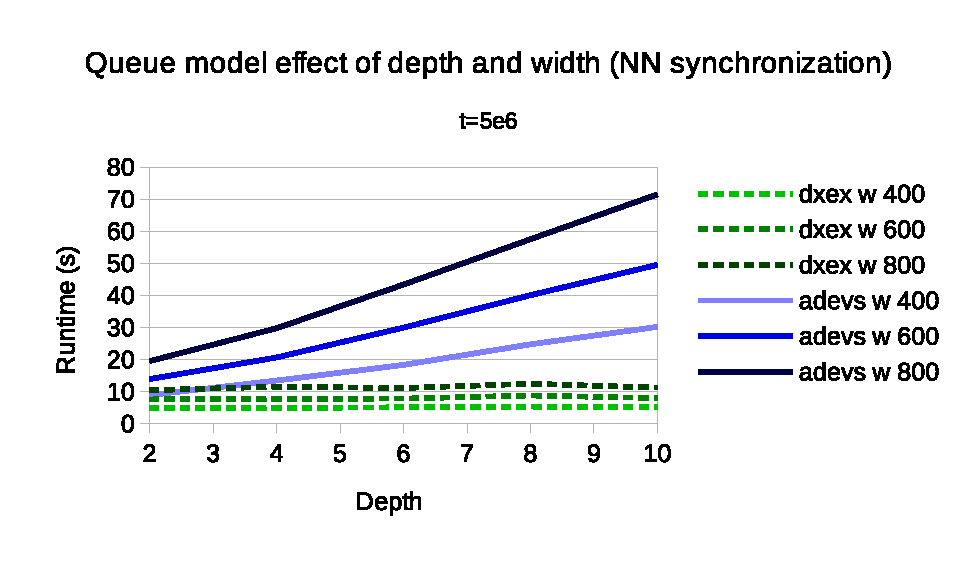
\includegraphics[width=\plotfraction\columnwidth]{fig/queue_fixed_sequential.eps}
	\caption{Queue benchmark results for sequential simulation.}
	\label{fig:Queue_benchmark_seq}
\end{figure}
\subsubsection{Interconnect}\label{4-seq-Interconnect}
In the Interconnect model, we increase the number of atomic models, thus quadratically increasing the number of couplings and the number of external transitions.
As can be seen in Figure~\ref{fig:Interconnect_benchmark}, adevs outperforms dxex by a fair margin.
Analysis showed that this is caused by the high amount of exchanged events: event creation is much slower in dxex than it is in adevs, despite dxex's use of memory pools. Dxex reuses the same event type for all synchronization algorithms. To shield the user from threading and deallocation concerns dxex provides an event superclass from which the user can derive to create a specialized event type. Copying and deallocation semantics are solved by the kernels at a runtime cost in simulations where event frequency is very high. Profiling the diverging benchmarks clearly shows the increasing cost of output generation (event creation) and deallocation as the determining factor in the gap in performance. We refer the interested reader to the dxex \hyperref{https://bitbucket.org/bcardoen/devs-ex-machina}{}{repo}{repository} for the profiling call graphs for the different benchmarks.


\begin{figure}
	\center
	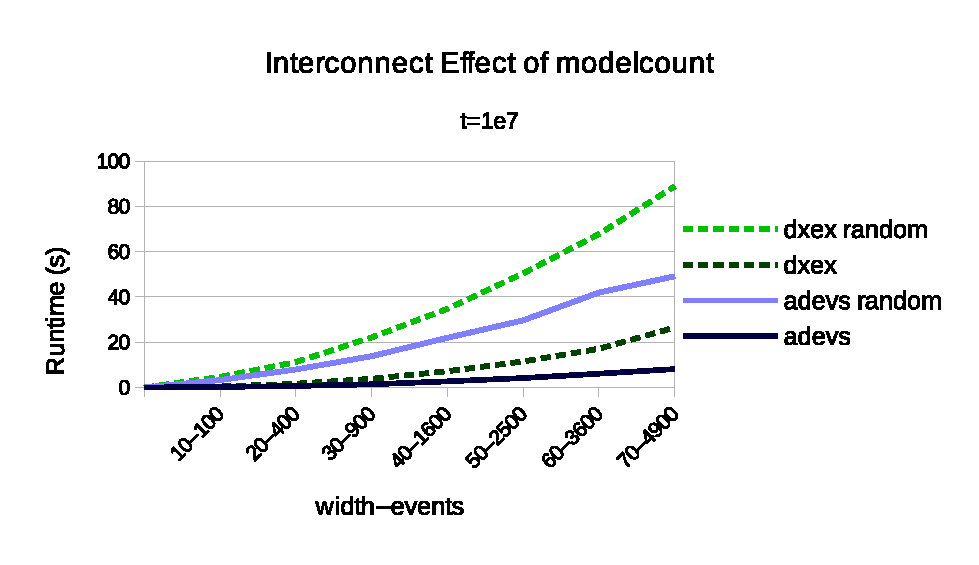
\includegraphics[width=\plotfraction\columnwidth]{fig/interconnect_sequential.eps}
	\caption{Interconnect benchmark results for sequential simulation.}
	\label{fig:Interconnect_benchmark}
\end{figure}
% We want to show the effect of message storms, that dxex is sensitive to this (even with allocators)
\subsubsection{PHold}\label{4-seq-PHold}
% Phold : difference with interconnect, less messages == equal performance dxex adevs
The PHold model is very similar to the Interconnect model. The biggest difference is that the amount of messages sent is much lower. The number of events scales linear with the number of models, not quadratic. Figure~\ref{fig:Phold_benchmark} shows that the performance of dxex and adevs are very close to each-other, with adevs slightly outperforming dxex.
\begin{figure}
	\center
	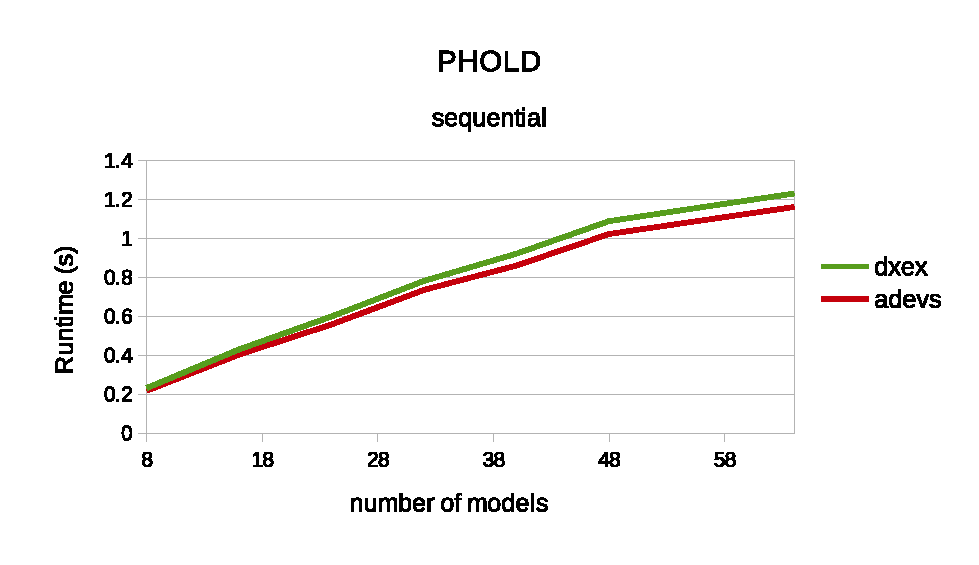
\includegraphics[width=\plotfraction\columnwidth]{fig/phold_sequential.eps}
	\caption{PHold benchmark results for sequential simulation.}
	\label{fig:Phold_benchmark}
\end{figure}
\subsubsection{PHoldTree}
The PHoldtree, like Queue, is a highly hierarchical model but one where the flattened structure cannot be partitioned into a chain as in Queue.
This topology is interesting since it highlights the effects of allocation which we have shown already in PHold and Interconnect to be of vital importance. This model allows us to investigate in depth the effects of non-cyclic allocation strategies and measure parallel speedup.\\
Since adevs does not use the directconnect algorithm, we expect some performance penalty between dxex and adevs. Conversely the messaging intensity in PHoldTree can be configured to highlight dxex's performance disadvantage in  benchmarks with a high event frequency as shown in the Interconnect benchmark.
\paragraph*{Event frequency}
Similarly when the probability on a priority message (p) increases the amount of messages generated will increase and thus the runtime. In Figure \ref{fig:PHoldtree_seq_p_benchmark} we observe that the messaging probability has a near linear impact on performance, with the shape of the curve due to rounding errors. The advantage adevs has in simulations where event frequency is high has been demonstrated by the interconnect benchmark. Dxex chooses to provide the user with an event type where the user need not consider deallocation or copy semantics, at a cost in performance where event frequency is high. Counterintuitively the probability of a high priority event in this model does not affect the performance difference between conservative and optimistic. The key parameter quickly becomes the load of a kernel in models. Our conservative implementation in an uncertain (trivial lookahead) simulation is very sensitive to a high load in models, whereas optimistic has no such limitation.
\paragraph*{Hierarchy}
To establish a performance baseline for the parallel simulation benchmarks we instrument how the PHoldTree benchmark performs sequential when we vary each of the model's parameters. 
When we increase the depth and fanout of the model, we expect to see an increase in runtime. In Figure \ref{fig:PHoldtree_seq_dn_benchmark} the n parameter (fanout) determines the performance penalty adevs suffers w.r.t dxex but we need to look at the profiling call graphs to determine what causes adevs' performance graph to behave non linear. \\
If we compare the instances d=2, n=2 with d=2, n=4 which show a clear deviation in performance between adevs and dxex for the latter, we conclude that the increase in width per subtree (n) leads to higher overhead for adevs. Dxex in contrast due to the directconnect algorithm has no such overhead. The intuition behind this effect, and especially why the d parameter does not have such an impact, is that an increase in n will rapidly increase the number of connections \ref{eq:pholdtreelinkcount} (and thus the routing problem adevs faces), whereas d will increase modelcount \ref{eq:pholdtreemodelcount} faster but have a lesser impact on connections. Both kernels scale linear in increasing number of atomic models. 
\begin{figure}
	\center
	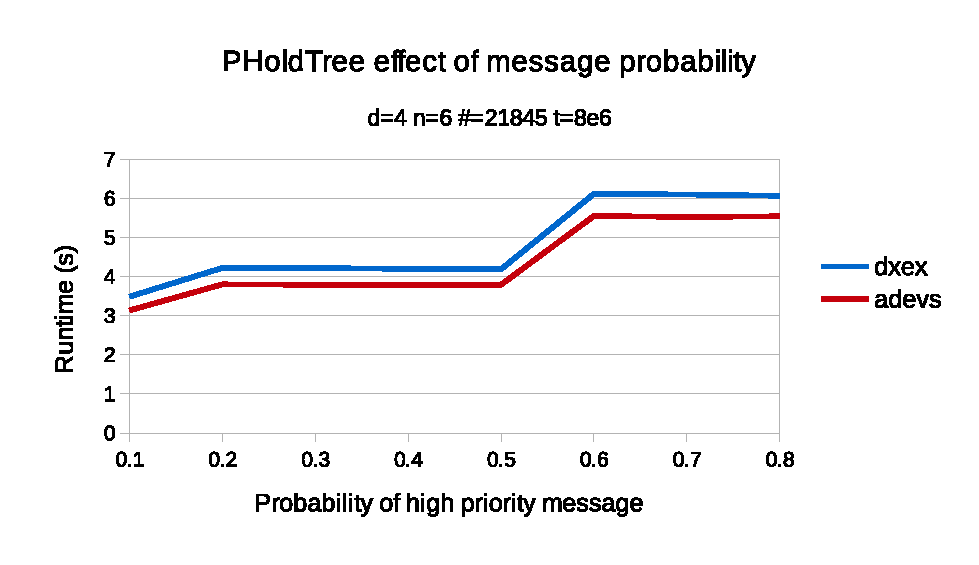
\includegraphics[width=\plotfraction\columnwidth]{fig/pholdtree_sequential_p.eps}
	\caption{PHoldTree for increasing probability of priority message.}
	\label{fig:PHoldtree_seq_p_benchmark}
\end{figure}
% Img for p increasing
\begin{figure}
	\center
	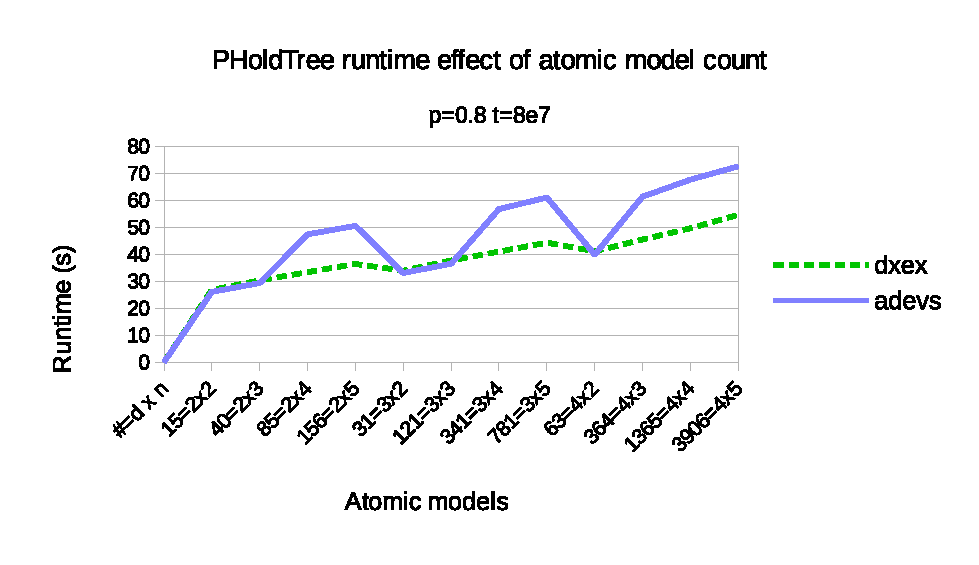
\includegraphics[width=\plotfraction\columnwidth]{fig/pholdtree_sequential_dn.eps}
	\caption{PHoldTree : Effect of hierarchy.}
	\label{fig:PHoldtree_seq_dn_benchmark}
\end{figure}